\documentclass[12pt,a4paper]{article}\usepackage[]{graphicx}\usepackage[]{xcolor}
% maxwidth is the original width if it is less than linewidth
% otherwise use linewidth (to make sure the graphics do not exceed the margin)
\makeatletter
\def\maxwidth{ %
  \ifdim\Gin@nat@width>\linewidth
    \linewidth
  \else
    \Gin@nat@width
  \fi
}
\makeatother

\definecolor{fgcolor}{rgb}{0.345, 0.345, 0.345}
\newcommand{\hlnum}[1]{\textcolor[rgb]{0.686,0.059,0.569}{#1}}%
\newcommand{\hlsng}[1]{\textcolor[rgb]{0.192,0.494,0.8}{#1}}%
\newcommand{\hlcom}[1]{\textcolor[rgb]{0.678,0.584,0.686}{\textit{#1}}}%
\newcommand{\hlopt}[1]{\textcolor[rgb]{0,0,0}{#1}}%
\newcommand{\hldef}[1]{\textcolor[rgb]{0.345,0.345,0.345}{#1}}%
\newcommand{\hlkwa}[1]{\textcolor[rgb]{0.161,0.373,0.58}{\textbf{#1}}}%
\newcommand{\hlkwb}[1]{\textcolor[rgb]{0.69,0.353,0.396}{#1}}%
\newcommand{\hlkwc}[1]{\textcolor[rgb]{0.333,0.667,0.333}{#1}}%
\newcommand{\hlkwd}[1]{\textcolor[rgb]{0.737,0.353,0.396}{\textbf{#1}}}%
\let\hlipl\hlkwb

\usepackage{framed}
\makeatletter
\newenvironment{kframe}{%
 \def\at@end@of@kframe{}%
 \ifinner\ifhmode%
  \def\at@end@of@kframe{\end{minipage}}%
  \begin{minipage}{\columnwidth}%
 \fi\fi%
 \def\FrameCommand##1{\hskip\@totalleftmargin \hskip-\fboxsep
 \colorbox{shadecolor}{##1}\hskip-\fboxsep
     % There is no \\@totalrightmargin, so:
     \hskip-\linewidth \hskip-\@totalleftmargin \hskip\columnwidth}%
 \MakeFramed {\advance\hsize-\width
   \@totalleftmargin\z@ \linewidth\hsize
   \@setminipage}}%
 {\par\unskip\endMakeFramed%
 \at@end@of@kframe}
\makeatother

\definecolor{shadecolor}{rgb}{.97, .97, .97}
\definecolor{messagecolor}{rgb}{0, 0, 0}
\definecolor{warningcolor}{rgb}{1, 0, 1}
\definecolor{errorcolor}{rgb}{1, 0, 0}
\newenvironment{knitrout}{}{} % an empty environment to be redefined in TeX

\usepackage{amsmath}
\usepackage{alltt}
\pdfoptionpdfminorversion=6 %para parar o erro "PDF inclusion: found PDF version<1.6>, but at most version<1.5> allowed"
\usepackage[T1]{fontenc}% Pacote para usar fontes escalonáveis
\usepackage[brazil]{babel}% Pacote para usar português
\usepackage[utf8]{inputenc}% Pacote para poder usar acentuação no arquivo.tex
\usepackage{float}%Utilizar float antes de hyperref elimina: destination with the same identifier...
%https://tex.stackexchange.com/questions/18924/pdftex-warning-ext4-destination-with-the-same-identifier-nam-epage-1-has
\usepackage[pdfpagelabels]{hyperref}
\hypersetup{colorlinks=true,allcolors=black}
\usepackage{amsmath}%
\usepackage{amsthm}%
\usepackage{amssymb}
\usepackage[alf,abnt-emphasize=bf,abnt-etal-list=5]{abntex2cite}

\usepackage[shortlabels,inline]{enumitem}
\renewcommand{\thesection}{\arabic{section}}
\usepackage{xcolor}
\usepackage{indentfirst}
\IfFileExists{upquote.sty}{\usepackage{upquote}}{}
\begin{document}
\pagenumbering{arabic} 
\pagestyle{plain} 





\begin{center}
\textbf{\Large Modelagem da diferença de gols por distribuições discretas: uma aplicação ao Campeonato Brasileiro}\\
\end{center} 
\begin{center}
\textbf{Eu da Silva$^{1}$; Kamilla Andrade de Oliveira$^{2}$; Paulo César Emiliano$^{3}$.}
\end{center}

1 Eu da Silva; Universidade Federal de XXX, Departamento de XXX; xxx@xxx.com.br

2 Kamilla Andrade de Oliveira; Universidade Federal do Maranhão, Departamento de Engenharia Agrícola, kamilla.andrade@ufma.br 

3 Paulo César Emiliano; Universidade Federal de Viçosa, Departamento de Estatística; paulo.emiliano@ufv.br


\begin{center}
    \textbf{Resumo}
\end{center}
\vspace{-.3cm}

\noindent 
A diferença entre o número de gols marcados por mandantes e visitantes constitui uma variável discreta de interesse em estudos sobre desempenho esportivo, refletindo o efeito agregado do mando de campo ao longo das rodadas de uma competição. Neste trabalho, foram comparados quatro modelos probabilísticos discretos para descrever a distribuição dessa variável: a distribuição normal discreta, a distribuição \textit{skew}--normal discreta, a distribuição de Skellam e a distribuição da diferença Weibull discreta. Foram analisadas 760 rodadas do Campeonato Brasileiro da Série A, compreendendo o período de 2006 a 2025. Os parâmetros dos modelos foram estimados pelo método da máxima verossimilhança, e a qualidade do ajuste foi avaliada por meio dos critérios de informação de Akaike (AIC) e bayesiano (BIC), além da inspeção gráfica das probabilidades ajustadas e das frequências observadas. A análise descritiva indicou uma distribuição aproximadamente simétrica, com média de 4,89 gols, baixa assimetria e leve excesso de curtose. Entre os modelos avaliados, a distribuição de Skellam apresentou os menores valores de AIC e BIC, evidenciando o melhor equilíbrio entre qualidade de ajuste e parcimônia. Os resultados mostram que, embora todos os modelos reproduzam adequadamente a região central da distribuição, a distribuição de Skellam fornece a representação probabilística mais adequada para a diferença de gols por rodada, além de possuir interpretação compatível com a natureza dos dados de contagem que originam essa variável.

\vspace{.4cm}
 
\noindent
\textbf{Palavras-chaves}: distribuição de Skellam; distribuição normal discreta; máxima verossimilhança; modelagem de contagens.
 \vspace{1cm}

\begin{center}
\textbf{Abstract}
\end{center}

\vspace{-.3cm}
The difference between the number of goals scored by home and away teams is a discrete variable of interest in sports performance studies, reflecting the aggregate home-field advantage throughout the rounds of a competition. In this study, four discrete probabilistic models were compared to describe the distribution of this variable: the discrete normal distribution, the discrete skew-normal distribution, the Skellam distribution, and the discrete Weibull difference distribution. A total of 760 rounds from the Brazilian Série A Championship, covering the period from 2006 to 2025, were analyzed. Model parameters were estimated by the maximum likelihood method, and goodness of fit was assessed using the Akaike Information Criterion (AIC) and the Bayesian Information Criterion (BIC), as well as graphical comparisons between fitted probabilities and observed frequencies. Descriptive analysis indicated an approximately symmetric distribution, with a mean of 4.89 goals, negligible skewness, and a slight excess of kurtosis. Among the models considered, the Skellam distribution achieved the lowest AIC and BIC values, indicating the best balance between goodness of fit and parsimony. The results show that, although all models adequately reproduce the central region of the distribution, the Skellam distribution provides the most appropriate probabilistic representation of the goal difference per round, while also offering an interpretation that is consistent with the count-data generating process underlying this variable.

\vspace{.4cm}
 
\noindent \textbf{Keywords}: Skellam distribution; discrete normal distribution; maximum likelihood; count data modeling.

\newpage

\section{Introdução}

\indent\par De acordo com o COB (\citeyear{cob2026}) o futebol é um dos esportes mais populares do mundo e tem suas origens mais remotas ligadas à China, mas foi na Inglaterra do século XIV que começou a tomar sua forma atual. O futebol foi introduzido no Brasil no final do século XIX, por imigrantes ingleses que trabalhavam nas ferrovias, os quais fundaram os primeiros clubes de futebol. De acordo com Recife (\citeyear{sport2024}) desde este período, passando por todo o século XX e agora entrando no século XXI, a história brasileira tem no futebol um importante ator. O futebol se tornou o esporte mais popular do Brasil criando uma verdadeira paixão nacional, que atravessa gerações e faz do futebol uma parte inseparável da identidade brasileira.

O Campeonato Brasileiro de Futebol é a principal competição nacional da modalidade no Brasil, sendo também considerada uma das ligas mais competitivas do mundo. 
Segundo Cordeiro et al. (\citeyear{Cordeiro2023}) o campeonato constitui-se em uma competição nacional equilibrada, com menores distâncias de pontuação entre os primeiros colocados e maior alternância de equipes campeãs. Uma realidade observada nos últimos anos, é a alternância entre Palmeiras e Flamengo como as equipes campeãs e a permanência deste cenário em um futuro próximo, principalmente devido a fatores econômicos, pode ser uma realidade (Relatório Convocados, \citeyear{Convocados2026}).

Brazão (\citeyear{Brazao2016}) pontua que nos primórdios, acreditava-se que o objetivo do futebol era marcar gols, hoje em dia, o futebol se preocupa cada vez mais em não sofrer gols. Segundo as estatísticas da CBF (CBF, \citeyear{CBF2026MediaGols}), a última vez em que o campeonato brasileiro superou a marca de mil gols em uma edição foi em 2011 e, a média de gols por partida superou 2,5 somente em 2025.

Diversas pesquisas foram elaboradas com o intuito de estudar o número de gols marcados, tais como Karlis e Ntzoufras (\citeyear{Karlis2003}) que utilizaram a distribuição Poisson bivariada para descrever o número de gols marcados por duas equipes e com esta distribuição conseguiram capturar a dependência e promover melhoria nos resultados com  empates; Karlis e Ntzoufras (\citeyear{Karlis2009}) que propuseram modelar diretamente a diferença de gols utilizando a distribuição Skellam e sob enfoque bayesiano; Brojanigo (\citeyear{brojanigo2013analysis}) compara, dentre outros, a distribuição de Skellam com a distribuição normal discreta para modelar a diferença de gols em partidas de futebol; Boshnakov, Kharrat e McHale (\citeyear{boshnakov2017}) substituem a distribuição de Poisson bivariada pela Weibull bivariada discreta utilizando assim uma distribuição de contagem mais flexível. Os trabalhos supracitados utilizam, por vezes, covariáveis, tais como força da equipe, mando de campo, chutes a gol, número de faltas, número de cartões, etc.

O presente estudo tem por objetivo modelar a diferença entre o número de gols do mandante e do visitante em cada rodada do Campeonato Brasileiro utilizando as distribuições normal discreta, \textit{skew}--normal discreta, diferença Weibull discreta e Skellam, no intuito de verificar qual distribuição probabilística modela melhor a diferença de gols por rodada no Campeonato Brasileiro entre as temporadas de 2006 e 2025.
\section{Referencial teórico}

A modelagem estatística de resultados em partidas de futebol tem recebido crescente atenção nas últimas décadas em razão de suas aplicações em previsão de resultados, avaliação de desempenho de equipes, definição de estratégias esportivas e precificação de mercados de apostas. A natureza discreta da variável ``número de gols'' faz com que distribuições de probabilidade para dados de contagem sejam amplamente empregadas na literatura, destacando-se inicialmente os modelos baseados na distribuição de Poisson.

Os primeiros trabalhos assumiam que o número de gols marcados pelas equipes mandante e visitante seguia distribuições de Poisson independentes, permitindo a obtenção de probabilidades para cada placar possível. Embora essa abordagem apresente simplicidade matemática e facilidade de interpretação, ela pressupõe igualdade entre média e variância, hipótese que nem sempre é observada em competições de futebol. Dessa forma, diversos estudos passaram a propor extensões capazes de acomodar dependência entre os gols das equipes, superdispersão e outras características observadas nos dados.

Nesse contexto, Maher (\citeyear{maher1982}) propôs um dos primeiros modelos estatísticos para previsão de resultados no futebol utilizando regressão de Poisson para representar a força ofensiva e defensiva das equipes. Posteriormente, Dixon e Coles (\citeyear{Dixon1997}) aperfeiçoaram essa abordagem ao incorporar dependência entre placares de baixa contagem, melhorando significativamente o ajuste para partidas com poucos gols, característica recorrente em campeonatos nacionais.

Uma alternativa importante consiste em modelar diretamente a diferença entre o número de gols das equipes, em vez de modelar separadamente os gols do mandante e do visitante. Essa estratégia reduz a dimensionalidade do problema, elimina a necessidade de modelar conjuntamente duas variáveis de contagem e permite trabalhar diretamente com a variável responsável por determinar o resultado final da partida. Além disso, a diferença de gols apresenta interpretação esportiva imediata, sendo positiva em vitórias do mandante, nula em empates e negativa em vitórias do visitante. Karlis e Ntzoufras (\citeyear{Karlis2009}) demonstraram que, assumindo independência entre os gols das equipes e distribuições de Poisson marginais, a diferença de gols segue naturalmente uma distribuição de Skellam, fornecendo uma fundamentação probabilística para essa abordagem.

A distribuição de Skellam constitui, portanto, uma das principais ferramentas para modelar diferenças entre variáveis de contagem independentes. Sejam \(X \sim \text{Poisson}(\lambda_1)\) e \(Y \sim \text{Poisson}(\lambda_2)\), independentes, então \(D=X-Y\) segue uma distribuição de Skellam, cuja função de probabilidade depende apenas dos parâmetros \(\lambda_1\) e \(\lambda_2\). A principal vantagem desse modelo é sua interpretação probabilística direta, uma vez que preserva a estrutura da modelagem baseada em Poisson e permite calcular probabilidades para qualquer diferença de gols observada.

Entretanto, a distribuição de Skellam herda parte das limitações da distribuição de Poisson, principalmente quando os dados apresentam dispersão superior ou inferior à esperada. Essa limitação motivou o desenvolvimento de modelos alternativos capazes de representar distribuições discretas mais flexíveis. Entre essas alternativas destacam-se as distribuições Weibull discretas, que introduzem parâmetros adicionais capazes de controlar simultaneamente localização e dispersão dos dados, produzindo melhor ajuste em diferentes cenários de contagem. Boshnakov, Kharrat e McHale (\citeyear{boshnakov2017}) propuseram um modelo bivariado baseado na distribuição Weibull discreta para previsão de placares de futebol, demonstrando que distribuições mais flexíveis podem superar modelos clássicos de Poisson em termos de ajuste e capacidade preditiva.

Embora o modelo de Boshnakov, Kharrat e McHale (\citeyear{boshnakov2017}) seja formulado para os gols das equipes mandante e visitante, a mesma ideia pode ser estendida para a diferença de gols por meio da convolução entre duas distribuições Weibull discretas independentes. Nessa abordagem, a diferença entre as variáveis discretas representa uma generalização natural da distribuição de Skellam, substituindo as distribuições marginais de Poisson por distribuições Weibull discretas, capazes de acomodar diferentes níveis de dispersão.

Outra alternativa consiste na utilização da distribuição normal discreta. Obtida pela discretização da distribuição normal contínua, essa distribuição preserva as propriedades de simetria e simplicidade computacional da normal, sendo particularmente adequada quando a variável de interesse assume valores inteiros distribuídos em torno de um valor médio. Sua flexibilidade torna-a uma candidata natural para modelar diferenças de gols, principalmente em campeonatos com grande número de observações, nos quais o comportamento empírico da variável aproxima-se de uma distribuição aproximadamente simétrica.

Entretanto, distribuições simétricas podem não representar adequadamente situações em que existe assimetria na diferença de gols, fenômeno frequentemente observado em competições nas quais o fator mando de campo exerce influência significativa sobre os resultados. Nesses casos, a distribuição \textit{skew}--normal discreta surge como uma extensão da normal discreta ao incorporar um parâmetro adicional responsável por controlar a assimetria, permitindo representar distribuições deslocadas para a direita ou para a esquerda sem perder as propriedades fundamentais da família normal.

Brojanigo (\citeyear{brojanigo2013analysis}) comparou modelos baseados nas distribuições Skellam e normal discreta para a modelagem da diferença de gols, concluindo que a modelagem direta dessa variável constitui uma alternativa eficiente à modelagem dos placares completos. Além disso, o autor mostrou que, sob determinadas parametrizações, modelos baseados na distribuição normal discreta podem apresentar desempenho comparável ou superior ao modelo de Skellam, reforçando a importância da escolha adequada da distribuição probabilística para representar a diferença de gols.

Apesar da extensa literatura sobre previsão de resultados no futebol, poucos estudos investigam especificamente qual distribuição probabilística melhor descreve a diferença de gols em competições nacionais de longa duração. O Campeonato Brasileiro da Série A apresenta características que justificam essa investigação, como elevado número de partidas, equilíbrio competitivo entre as equipes, presença do fator mando de campo e variabilidade dos resultados ao longo das temporadas.

Diante desse contexto, o presente estudo tem por objetivo modelar a diferença entre o número de gols do mandante e do visitante em cada partida do Campeonato Brasileiro da Série A utilizando as distribuições normal discreta (Seção~\ref{sec:norm}), \textit{skew}--normal discreta (Seção~\ref{sec:snorm}), Skellam (Seção~\ref{sec:skel}) e diferença Weibull discreta (Seção~\ref{sec:weib}). A partir dos jogos realizados entre as temporadas de 2006 e 2025, pretende-se comparar o desempenho dessas distribuições por meio de critérios de qualidade de ajuste, como log-verossimilhança, Critério de Informação de Akaike (AIC) (Akaike, \citeyear{Akaike1974}) e Critério de Informação Bayesiano (BIC) (Schwarz, \citeyear{Schwarz1978}), identificando qual modelo probabilístico descreve de forma mais adequada a distribuição da diferença de gols observada na competição.

%Com o objetivo de identificar a distribuição probabilística mais adequada para modelar a diferença entre o número de gols marcados pelos clubes mandantes e visitantes em cada rodada do Campeonato Brasileiro da Série A, foram ajustados aos dados quatro modelos probabilísticos: a Normal discreta, a \textit{skew}--normal discreta, a distribuição de Skellam e a distribuição da diferença de Weibull discreta.

%%%%%%%%%%%%%%%%%%%%%%%%%%%%
\subsection{Distribuições probabilísticas para diferenças de contagens}

A modelagem da diferença entre o número de gols do mandante e do visitante pode ser realizada por diferentes distribuições probabilísticas definidas sobre o conjunto dos números inteiros. A escolha da distribuição depende das propriedades observadas nos dados, como simetria, assimetria, dispersão e comportamento das caudas. Nesta seção são apresentadas as distribuições utilizadas neste estudo.

\subsubsection{Distribuição normal discreta}\label{sec:norm}
Segundo Roy (\citeyear{Roy2003}), dada uma variável contínua com função de sobrevivência $S(x)$, podemos definir uma variável discreta $X$, com função de probabilidade 
$P[X=x]=\begin{cases}
S(x)-S(x+1),&x\in\mathbb{Z}\\
0,&\text{caso contrário.}
\end{cases}$ No caso em que \(X\) é uma variável aleatória com distribuição normal contínua de média \(\mu\) e variância \(\sigma^2\), isto é, $X\sim N(\mu,\sigma^2)$ com função distribuição acumulada $\Phi_X(\cdot)$, a função de probabilidade da distribuição normal discreta é dada por
\[
P[X=x]=
\Phi\left(\frac{x-\mu+1}{\sigma}\right)
-
\Phi\left(\frac{x-\mu}{\sigma}\right),
\qquad
x\in\mathbb{Z}.
\]
\subsubsection{Distribuição \textit{skew}--normal discreta}\label{sec:snorm}
A distribuição \textit{skew}-normal contínua, proposta por Azzalini (\citeyear{azzalini1985}) tem função densidade de probabilidade dada por
\[
f(x)=
\frac{2}{\lambda}
\phi\left(\frac{x-\mu}{\sigma}\right)
\Phi\left(
\lambda\frac{x-\mu}{\sigma}
\right),
\]
em que \(\phi(\cdot)\) e \(\Phi(\cdot)\) representam, respectivamente, a função densidade e a função distribuição acumulada da normal padrão, enquanto \(\mu\), \(\sigma>0\) e \(\lambda\) correspondem aos parâmetros de localização, escala e assimetria. A distribuição \textit{skew}--normal discreta é obtida por
$P[X=x]=F(x+1)-F(x)$, $x\in\mathbb{Z}$, em que \(F(\cdot)\) representa a função distribuição acumulada da distribuição \textit{skew}-normal contínua.

\subsubsection{Distribuição de Skellam}\label{sec:skel}
A distribuição de Skellam (Skellam, \citeyear{skellan1946}) é a distribuição exata da diferença entre duas variáveis aleatórias independentes com distribuição de Poisson. Sejam $X\sim\text{Poi}(\lambda_1)$ e $Y\sim\text{Poi}(\lambda_2)$, com \(X\) e \(Y\) independentes, então $D=X-Y\sim\text{Skellam}(\lambda_1,\lambda_2)$, cuja função de probabilidade é dada por
\[
P[D=d]=
e^{-(\lambda_1+\lambda_2)}
\left(
\frac{\lambda_1}{\lambda_2}
\right)^{d/2}
I_{|d|}
\left(
2\sqrt{\lambda_1\lambda_2}
\right),
\qquad
d\in\mathbb{Z},
\]
em que \(I_{d}(\cdot)\) denota a função de Bessel modificada de primeira espécie de ordem \(d\).

%A distribuição de Skellam apresenta interpretação probabilística direta para diferenças de gols, uma vez que os parâmetros \(\lambda_1\) e \(\lambda_2\) correspondem às médias das distribuições de gols do mandante e do visitante, respectivamente.

\subsubsection{Distribuição diferença Weibull discreta}\label{sec:weib}

Uma alternativa à distribuição de Skellam consiste em substituir as distribuições marginais de Poisson por distribuições Weibull discretas, permitindo maior flexibilidade para representar diferentes níveis de dispersão. Sejam $X\sim DW(q_1,\beta_1)$ e $Y\sim DW(q_2,\beta_2)$, variáveis aleatórias independentes, em que \(DW(\cdot)\) denota a distribuição Weibull discreta de Nakagawa e Osaki (\citeyear{Nakagawa1975}) a qual possui função de probabilidade dada por
\[
P[X=x]=q^{x^{\beta}}-q^{(x+1)^{\beta}},\qquad x=\in\mathbb{N}
\]
com $0<q<1$ e $\beta>0$. 

Considerando $D=X-Y$, a distribuição da diferença Weibull discreta não tem expressão fechada para sua função de probabilidade, a qual pode ser obtida pela convolução das distribuições marginais da seguinte forma
\[
P[D=d]=\begin{cases}
\sum\limits_{k=0}^{+\infty}
P[X=k+d]
P[Y=k],&\text{ se }d\geq0,\\
\sum\limits_{k=0}^{+\infty}
P[X=k]
P[Y=k-d],&\text{ se }d<0.\\
\end{cases}
\]

%Sua principal vantagem consiste na maior flexibilidade para representar distribuições com superdispersão ou subdispersão, características frequentemente observadas em dados esportivos.
%%%%%%%%%%%%%%%%%%%%%%%%%%%%%%
\section{Resultados e discussão}
%\section{Aplicação aos dados do campeonato brasileiro 2006 a 2025}

Os dados foram obtidos de Duque (\citeyear{Duque2025}) e referem-se, dentre outras variáveis, ao número de gols marcados pelos mandantes e pelos visitantes em cada uma das 38 rodadas do campeonato brasileiro para os anos de 2006 a 2025. Ao efetuar a diferença entre estas variáveis obteve-se a variável sob estudo que é a diferença entre o número de gols marcados pelos mandantes e os visitantes. O período escolhido refere-se aos campeonatos que contaram com a presença de 20 equipes com 380 jogos por ano (exceção feita a 2016 que teve 379 jogos). 

\subsection{Estatísticas descritivas}
As estatísticas descritivas são dadas na Tabela~\ref{tab:descritiva}, as quais foram sumariadas no \textit{boxplot} dado na Figura~\ref{fig:boxplot}, sendo que todos os resultados foram obtidos no \textit{software} R (R, \citeyear{R2026}). Verifica-se que a diferença média de gols por rodada foi de 4,8882 gols, valor muito próximo da mediana (5  gols) e, também, do desvio-padrão (4,91 gols), sugerindo uma distribuição aproximadamente simétrica em torno de seu centro. Essa percepção é corroborada pelo coeficiente de assimetria (0,02), indicando praticamente ausência de assimetria.

\begin{table}[!ht]
\centering
\caption{Estatísticas descritivas da diferença de gols por rodada do Campeonato Brasileiro (2006--2025).}\label{tab:descritiva}
\begin{tabular}{lcccccccccc}
\hline
$n$ &
$\bar{X}$ &$Md(X)$ &$s(X)$&$X_{(1)}$ &$Q_1$ &$Q_3$ &$X_{(n)}$ & 
$A(X)$ &
$K(X)$\\
\hline
760 &
4,89 &
5 &
4,91 &
$-13$ &
2 &
8 &
22 &
0,02 &
3,36\\
\hline
\multicolumn{10}{p{0.95\textwidth}}{\scriptsize
\textit{Notação:} $n$ = número de observações;
$\bar{X}$ = média amostral;
$Md(X)$ = mediana;
$s(X)$ = desvio-padrão amostral;
$X_{(1)}$ = valor mínimo;
$Q_1$ = primeiro quartil;
$Q_3$ = terceiro quartil;
$X_{(n)}$ = valor máximo;
$A(X)$ = coeficiente de assimetria;
$K(X)$ = coeficiente de curtose.
}\\
\end{tabular}
\end{table}

\begin{figure}[!ht]
\centering
\begin{knitrout}
\definecolor{shadecolor}{rgb}{0.969, 0.969, 0.969}\color{fgcolor}
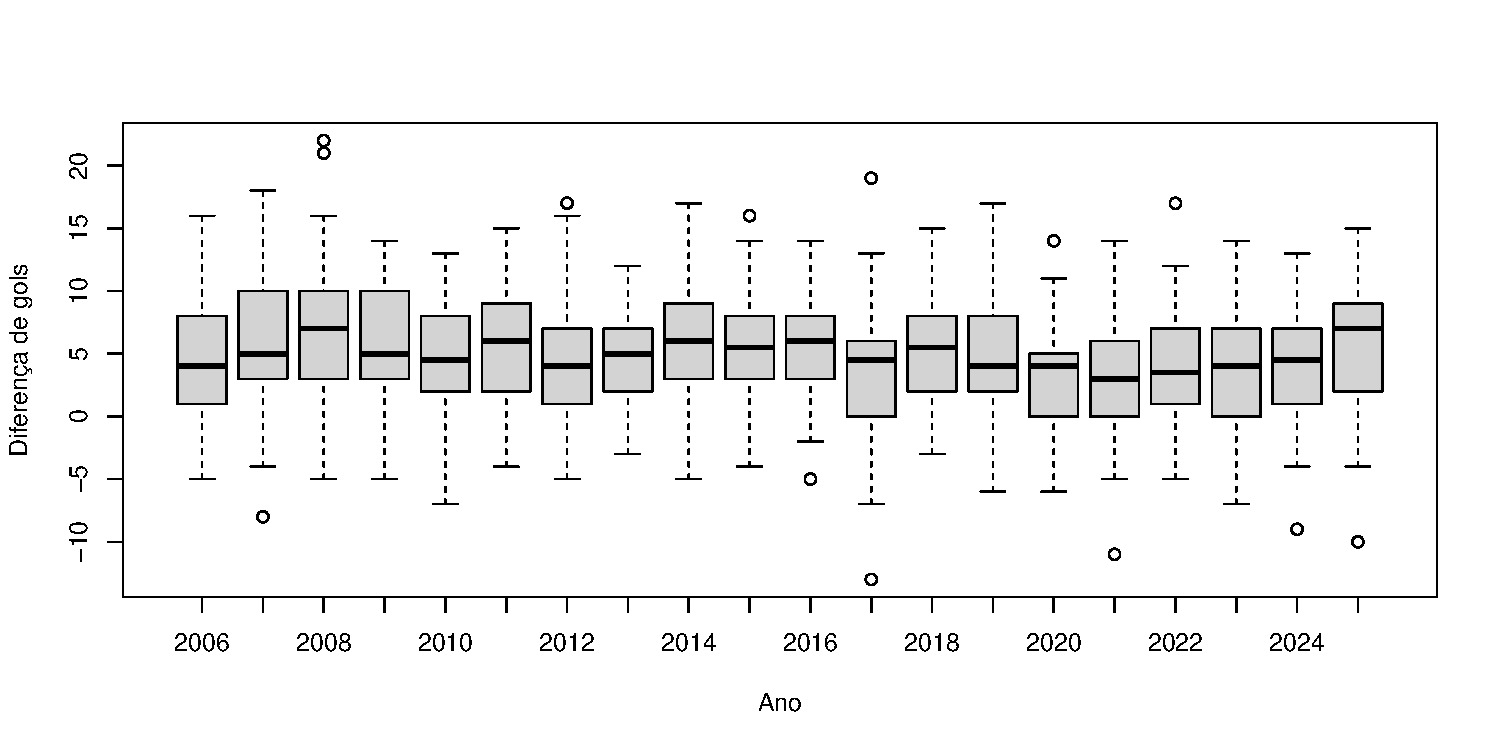
\includegraphics[width=\textwidth]{figure/boxplot-1} 
\end{knitrout}
\vspace{-1cm}
\caption{\textit{Boxplots} da diferença de gols por rodada segundo a temporada do Campeonato Brasileiro.}\label{fig:boxplot}
\end{figure}
%talvez um boxplot por rodada? 
%Ou  apresentar um boxplot de um ano específico?


A ocorrência de diferenças negativas ($X_{(1)}=-13$) demonstra que, em algumas rodadas, os clubes visitantes marcaram, no conjunto das partidas, mais gols do que os mandantes, tal fato só ocorreu em 96 rodadas das 760 analisadas. Em contrapartida, diferenças positivas elevadas $(X_{(n)}=22)$ evidenciam rodadas em que a vantagem do mando de campo foi bastante expressiva. A amplitude observada reforça a existência de rodadas atípicas, embora relativamente raras.

O coeficiente de curtose igual a 3,36 indica uma distribuição ligeiramente leptocúrtica em relação à distribuição normal, sugerindo maior concentração de observações próximas ao centro e uma probabilidade um pouco mais elevada de ocorrência de valores extremos. Esse comportamento é comum em variáveis derivadas de contagens e indica que modelos probabilísticos capazes de acomodar diferentes níveis de dispersão podem fornecer melhor ajuste aos dados.

Em conjunto, as estatísticas descritivas sugerem que a distribuição da diferença de gols por rodada apresenta comportamento aproximadamente simétrico, porém com variabilidade relativamente elevada e leve excesso de curtose. Essas características justificam a comparação entre diferentes distribuições discretas, como a Normal discreta, a \textit{skew}--normal discreta, a Skellam e a diferença de Weibull discreta, permitindo avaliar qual delas representa de forma mais adequada o comportamento probabilístico da diferença de gols observada no Campeonato Brasileiro.

\subsection{Distribuições ajustadas}
As distribuições sob estudo foram ajustadas aos dados de saldo de gols (mandante $-$ visitante) por rodadas para o campeonato brasileiro da série A nos anos de 2006 a 2025. Os parâmetros de cada distribuição foram estimados pelo método da máxima verossimilhança (MV), o qual consiste na obtenção dos valores dos parâmetros que maximizam a função de verossimilhança dos dados observados. Para os modelos normal discreta e Skellam foram utilizadas estimativas iniciais obtidas pelo método dos momentos, enquanto os parâmetros dos modelos \textit{skew}--normal discreta e diferença Weibull discreta foram obtidos por meio da maximização numérica da função de log-verossimilhança utilizando o algoritmo BFGS (\textit{Broyden--Fletcher--Goldfarb--Shanno}) (Fletcher, \citeyear{Fletcher1987}), amplamente empregado em problemas de otimização não linear.

A Tabela \ref{tab:parametros} apresenta as estimativas dos parâmetros obtidas pelo método da máxima verossimilhança para os quatro modelos probabilísticos considerados neste estudo. Os valores estimados permitem caracterizar diferentes aspectos da distribuição da diferença de gols entre mandantes e visitantes no Campeonato Brasileiro.

\begin{table}[!ht]
\centering
\caption{Estimativas dos parâmetros dos modelos ajustados.}
\label{tab:parametros}
\begin{tabular}{lccccc}
\hline
Normal discreta &
$\hat{\mu}=5,39$ &
$\hat{\sigma}=1,59$ &
-- &
-- \\

\textit{skew}--normal discreta &
$\hat{\mu}=3,24$ &
$\hat{\sigma}=5,35$ &
$\hat{\lambda}=0,58$ &
-- \\

Skellam &
$\hat{\lambda}_1=2,67$ &
$\hat{\lambda}_2=2,26$ &
-- &
-- \\

Diferença Weibull discreta &
$\hat{q}_1=5,01$ &
$\hat{\beta}_1=0,8$ &
$\hat{q}_2=1,57$ &
$\hat{\beta}_2=0,22$ \\
\hline
\end{tabular}
\end{table}

Na distribuição normal discreta, observa-se uma estimativa para a média de $\hat{\mu}=5,39$ e para o desvio padrão $\hat{\sigma}=1,59$. O valor estimado para $\hat{\mu}$ indica que a diferença de gols por rodada concentra-se em torno de valores positivos, sugerindo vantagem agregada dos mandantes. O parâmetro de dispersão relativamente reduzido indica menor variabilidade em torno desse valor central quando comparado aos demais modelos considerados.

A distribuição \textit{skew}--normal discreta apresenta estimativas de localização e escala dadas por $\hat{\mu}=3,24$ e $\hat{\sigma}=5,35$, respectivamente, além do parâmetro de assimetria $\hat{\lambda}=0,58$. O valor positivo do parâmetro de assimetria indica que esse modelo incorpora uma cauda mais alongada à direita, permitindo representar uma maior ocorrência de rodadas com diferenças elevadas de gols favoráveis aos mandantes. Além disso, a maior estimativa do parâmetro de escala em relação ao modelo normal discreto sugere maior flexibilidade para acomodar valores extremos da diferença de gols.

Para o modelo de Skellam, as estimativas obtidas foram $\hat{\lambda}_1=2,67$ e $\hat{\lambda}_2=2,26$. Esses parâmetros representam as médias das distribuições de Poisson associadas aos gols dos mandantes e visitantes, respectivamente. A diferença entre os parâmetros,
$\hat{\lambda}_1-\hat{\lambda}_2=0,41$, indica uma vantagem média esperada dos mandantes, resultado compatível com a característica histórica do futebol brasileiro, no qual as equipes mandantes tendem a apresentar maior desempenho ofensivo em seus estádios. Além disso, a proximidade entre os dois parâmetros evidencia equilíbrio entre os ataques das equipes mandantes e visitantes, característica incorporada naturalmente pela distribuição de Skellam.

Por fim, a distribuição da diferença Weibull discreta apresentou estimativas 
$\hat{q}_1=5,01$, $\hat{\beta}_1=0,8$, $\hat{q}_2=1,57$ e $\hat{\beta}_2=0,22$. Esses parâmetros permitem modelar separadamente as distribuições marginais associadas às contagens de gols dos mandantes e visitantes, antes da obtenção da diferença entre elas. Os diferentes valores dos parâmetros de forma indicam comportamentos distintos entre as duas distribuições marginais, sugerindo maior flexibilidade para capturar assimetrias e dispersões não representadas adequadamente pelos modelos baseados exclusivamente na normal ou na diferença de Poisson. Dessa forma, a distribuição Weibull discreta apresenta potencial para modelar situações em que a variabilidade das contagens de gols difere entre mandantes e visitantes.

A comparação apresentada na Tabela \ref{tab:criterios} evidencia que a distribuição de Skellam apresentou o menor valor de AIC (4578,4) e de BIC (4587,66), sendo, portanto, o modelo mais adequado segundo ambos os critérios de seleção. Esse resultado indica que a estrutura probabilística baseada na diferença entre duas variáveis de contagem com distribuição de Poisson foi capaz de representar satisfatoriamente o comportamento da diferença de gols por rodada no Campeonato Brasileiro, utilizando apenas dois parâmetros. As demais distribuições, embora apresentem mais parâmetros e, consequentemente possuem maior flexibilidade, não apresentaram melhoria suficiente na qualidade do ajuste que justifiquem sua escolha pois o modelo não é o mais parcimonioso. Esse resultado evidencia que modelos com maior número de parâmetros não necessariamente apresentam melhor capacidade descritiva quando o aumento da complexidade não é acompanhado por uma elevação significativa da verossimilhança.

\begin{table}[!ht]
\centering
\caption{Critérios de seleção dos modelos ajustados.}
\label{tab:criterios}
\begin{tabular}{lcccc}
\hline
Modelo &  AIC & BIC\\
\hline
Normal discreta & 4579,16 & 4588,43 \\
\textit{skew}--normal discreta & 4581,01 & 4594,91 \\
Skellam & 4578,4 & 4587,66 \\
Diferença Weibull discreta & 4580,07 & 4598,6\\
\hline
\end{tabular}
\end{table}


%Por outro lado, a inclusão do parâmetro de assimetria no modelo \textit{skew}--normal discreto não proporcionou melhoria no ajuste sugerindo que, para os dados analisados, a assimetria adicional incorporada pela distribuição \textit{skew}--normal não representa uma característica relevante da distribuição da diferença de gols. A distribuição de Skellam apresenta uma fundamentação probabilística mais adequada para variáveis originadas da diferença entre contagens, uma vez que a diferença de gols é construída a partir dos gols dos mandantes e visitantes.

%Comparando especificamente os modelos baseados em distribuições discretas simétricas e assimétricas, observa-se que a introdução de parâmetros adicionais de forma e assimetria não resultou em ganhos no ajuste. A diferença entre os valores dos critérios de informação indica que a estrutura dos dados pode ser adequadamente representada por modelos mais parcimoniosos. Da mesma forma, a comparação entre a distribuição de Skellam e a diferença Weibull discreta demonstra que, embora a última permita maior flexibilidade na modelagem das contagens marginais, a hipótese de diferença entre variáveis Poisson mostrou-se mais eficiente para representar a distribuição da diferença de gols observada.

%Utilizando-se os critérios AIC (round(AIC_skel,2)) e BIC (round(BIC_skel,2)), a distribuição de Skellam foi selecionada como o modelo mais adequado para caracterizar a diferença de gols entre mandantes e visitantes nas rodadas do Campeonato Brasileiro analisadas. 




A Figura \ref{fig:ajustes} apresenta as frequências empíricas da diferença de gols por rodada juntamente com as probabilidades estimadas pelos quatro modelos considerados.

\begin{figure}[!ht]
\centering
\begin{knitrout}
\definecolor{shadecolor}{rgb}{0.969, 0.969, 0.969}\color{fgcolor}
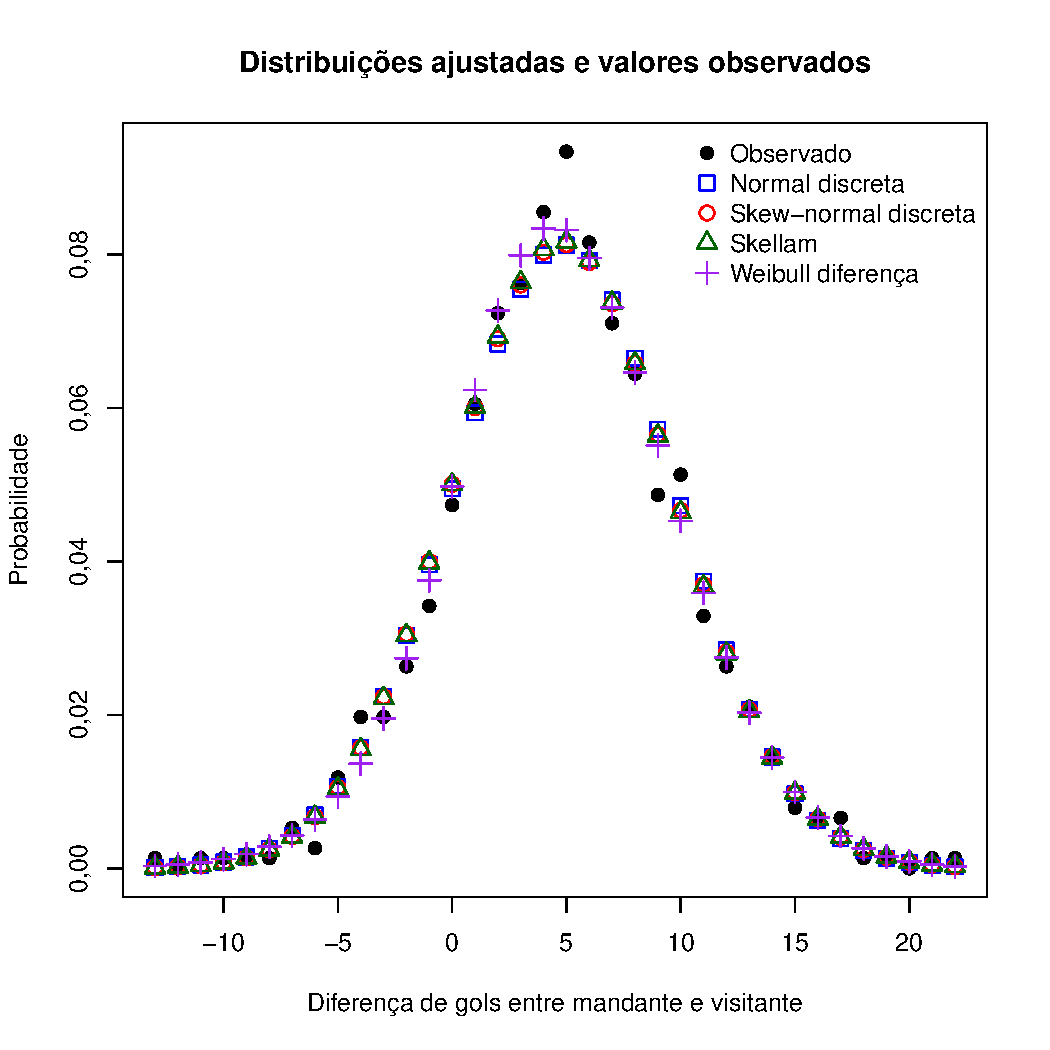
\includegraphics[width=\maxwidth]{figure/47THRCT2UniEsq-1} 
\end{knitrout}
\caption{Frequências observadas e probabilidades ajustadas pelos modelos probabilísticos.}
\label{fig:ajustes}
\end{figure}

Visualmente, observa-se que todas as distribuições conseguem reproduzir adequadamente a região central da distribuição, onde se concentra a maior parte das observações. Entretanto, diferenças importantes surgem na representação das caudas, responsáveis pelos valores extremos da diferença de gols.

\section{Conclusões}

Neste trabalho foram comparadas quatro distribuições discretas para modelar a diferença entre o número de gols marcados por mandantes e visitantes, agregada por rodada do Campeonato Brasileiro da Série A no período de 2006 a 2025. Inicialmente, a análise descritiva mostrou que a variável apresenta comportamento aproximadamente simétrico, média próxima da mediana, baixa assimetria e leve excesso de curtose, características que justificam a comparação entre modelos discretos com diferentes níveis de flexibilidade.

Os parâmetros dos modelos foram estimados pelo método da máxima verossimilhança e a comparação foi realizada por meio dos critérios de informação AIC e BIC. Entre os modelos considerados, a distribuição de Skellam apresentou os menores valores desses critérios, proporcionando equilíbrio entre qualidade de ajuste e parcimônia. Embora as diferenças em relação aos demais modelos sejam pequenas, o resultado sugere que a estrutura baseada na diferença entre duas variáveis de Poisson representa adequadamente a distribuição da diferença de gols por rodada.

Os resultados também evidenciam que o aumento do número de parâmetros não implica, necessariamente, melhora no desempenho do modelo. Apesar da maior flexibilidade das distribuições \textit{skew}--normal discreta e diferença Weibull discreta, seus ajustes não proporcionaram ganhos suficientes para compensar a maior complexidade, conforme indicado pelos critérios de informação.

Como perspectivas para trabalhos futuros, podem ser considerados modelos que relaxem a hipótese de independência entre os gols de mandantes e visitantes, bem como distribuições capazes de acomodar sobredispersão ou excesso de zeros, além da incorporação de covariáveis relacionadas às características das equipes, local da partida etc. Essas extensões poderão fornecer descrições ainda mais realistas da dinâmica de gols no futebol brasileiro.

\section*{Agradecimentos}
Os autores agradecem Capes, CNPq, Fapemig e a Universidade Federal de Viçosa que deram suporte financeiro para realização deste artigo.
\begin{flushleft}
%\begingroup
%\renewcommand{\bibsection}{}
%\section*{Referências bibliográficas}
%\addcontentsline{toc}{section}{REFERÊNCIAS}
\bibliography{Referencias}


%\endgroup
\end{flushleft}
\end{document} 
